\chapter{PoC 1: Ethereum dApp}\label{chapter:poc1}

\section{Introduction}
Existing applications for sharing files are central solutions and therefore suffer from single point of failure risk. Moreover, using central services for securing data means that we have to trust a 3rd party with our data thus exposing it to manipulation risks. Hence, a decentralized
application is required to overcome the problems posed by a central application. With the recent developments in Blockchain technology and P2P storage, it is possible to securely store and share data without using any central server.

This chapter describes the workings of the application \textit{dShare}\cite{harsh_kedia_2019_3359852} built using P2P technologies enabling a secure way of storing and sharing data between two individuals or entities. The latest version of the application is deployed at \url{https://file-share-dapp.herokuapp.com/}

\section{Technologies Used}

\subsection{Ethereum}
Ethereum\cite{buterin2014ethereum} is a blockchain platform for building decentralized applications. It allows the creation of \textit{Smart Contracts}. Solidity\footnote{\url{https://github.com/ethereum/solidity}} is the primary language for writing smart contracts on Ethereum.

\subsection{InterPlanetary File System (IPFS)}
IPFS\cite{benet2014ipfs} is a peer-to-peer file transfer protocol which enables a shared file system between all its connected peers. It achieves this by combining previous peer-to-peer systems such as Distributed Hash Tables (DHT), BitTorrent\cite{cohen2008bittorrent}, and Git\cite{loeliger2012version}. The data in the IPFS network are modeled as a Merkle DAG\footnote{Merkle directed acyclic graph - similiar to a Merkle tree data structure however they do not need to be balanced and it’s non-leaf nodes can contain some data.} thus providing a throughput storage system with content-addressed hyperlinks.

\begin{figure}[h]
	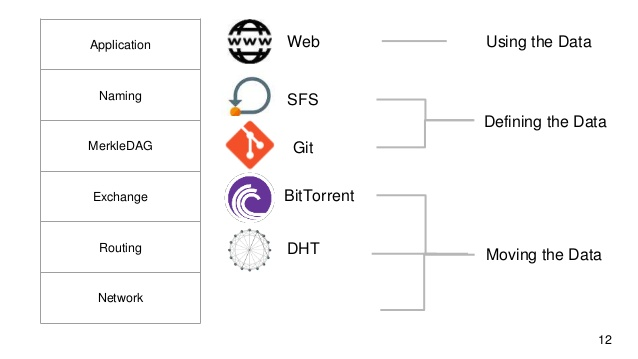
\includegraphics[width=\linewidth]{figures/ipfs-stack}
	\caption{\label{fig:ipfs-stack} IPFS Stack}
\end{figure}

Figure~\ref{fig:ipfs-stack}\footnote{Adopted from: \url{https://image.slidesharecdn.com/ipfs-171229085327/95/ipfs-12-638.jpg?cb=1514537643}} shows the IPFS Stack. It consists of sub-protocols, each providing a different functionality.

\begin{itemize}
	\item Identities - node identification and verification.
	\item Network - connection management among peers.
	\item Routing - peer lookup using DHT.
	\item Exchange - data exchange strategies among peers.
	\item Objects - a content-addressed Merkle DAG.
	\item Files - versioned file system.
	\item Naming - A self-certifying mutable name system.
\end{itemize}

\subsection{OriginStamp}
OriginStamp\cite{hepp2018originstamp} is a blockchain based system for decentralized timestamping. It uses the Bitcoin blockchain for the creation of trusted and immutable timestamps for any piece of data. Timestamps created by OriginStamp can be verified independently by anyone.

\begin{figure}[h]
	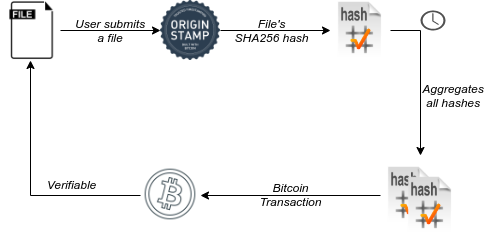
\includegraphics[width=\linewidth]{figures/origin-stamp}
	\caption{\label{fig:originstamp} Timestamping using OriginStamp}
\end{figure}

Figure~\ref{fig:originstamp} visualizes the timestamping process as implemented in OriginStamp. When a user submits a file, the hash of the data is recorded. It combines all the hashes submitted over a period of time and generates an aggregated hash. After some additional hashing and encoding operations, a Bitcoin address is created to which the smallest possible transactional amount of Bitcoins is transferred. Performing this transaction embeds the hash and the timestamp permanently to the Bitcoin blockchain. Each transaction is part of a block and is added to the Bitcoin blockchain by a process called mining. Since each block is linked cryptographically to the previous block, adding a new block confirms the validity of the last block. Changing the timestamp of a transaction becomes impossible once five or six subsequent blocks are mined, which requires an hour on average\cite{nakamoto2008bitcoin}.

\section{Implementation}
For storing of files we used IPFS. Before uploading to the IPFS network, files are encrypted using AES-GCM encryption mechanism. Sharing of encryption keys is facilitated using smart contracts built on Ethereum; thus files can be shared by anyone with an Ethereum address. Finally, OriginStamp is used for immutable timestamping.

The front-end of the application is built using React.js, a JavaScript library for building user interfaces. Solidity was used for writing smart contracts and deployed on the Ethereum test network, Rinkeby. Next.js was used for server-side rendering (SSR), and Firebase was used as a database for storing public Ethereum key of the users.

\section{Working}